%!TEX root = ../main.tex

\section{Pre-analysis} % (fold)
\label{sec:preanalysis}

For this semester we have chosen the theme \textit{Sonification}.
In researching sonification and audification, it was clear that there are more ways of sonifying data, depending on what kind of data is to be converted, how that information is to be displayed and interacted with. 
Weather information contains many different types of data. 
Some of these could be: \newline
temperature (degrees), sunny or cloudy (either or), wind speed (meters per second), visibility, precipitation (rain/sleet/snow/hail measured in millimeters). 
This means that theoretically a lot of different sonification techniques can be applied to this kind of information. 
Furthermore, we would like to investigate if visually presented weather data can actually be understood, and to which degree, if converted to non-speech sound using sonification. 
Can sonification of some of these data maybe even make the weather information more understandable or relatable? 
For instance, is information about wind or downpour more relatable as sound than numbers? These discussions have led us to the following Initial Problem Statement:


\subsection{Initial Problem Statement} % (fold)
\label{sub:initial_problem_statement}

Is it possible to successfully use sonification to convey relevant information about \newline 
weather conditions as efficiently as visually represented weather applications?

% subsection initial_problem_statement (end)


\subsection{Sonification} % (fold)
\label{sub:sonification}

Sonification is used to convey information through non-speech audio, to get a better understanding of what that is; 
we will explain what kind of communication methods there are and examples of their function (visualization, auditory and sonification).


Visualization is the communication method that we perceive through our eyes e.g. posters, TV, computer, traffic lights, chat systems, pictures, sign language, body language etc. relevant to our IPS, a weather application that shows a weather forecast.


Auditory communication is data that we perceive through our ears just like sonification, but unlike sonification, auditory communication can use speech, which occurs in for instance, radio, TV, computers, telephones, all kinds of equipment and applications that allow you talk with people over distance. 
Sonification only uses non-speech audio to convey information, an example is traffic light junctions all around Denmark. 
When you near a crosswalk you will hear 2 different sounds. 
Both sounds are the same, but they consist of different paces of rhythm. 
One sound (slow) indicates it’s a red light, while the other (fast) indicates it’s safe to walk. 
This helps blind people to know whether to cross or not, and is an example of sonification. 
Sonification is a subset of auditory displays\footnote{\textbf{Auditory display} is the use of sound to communicate information from a computer to the user \cite*{McGookin2004}}. 
There are several uses of sonification, and these will be described in detail below.

% subsection sonification (end)

\subsubsection{Examples of sonification} % (fold)
\label{ssub:examples_of_sonification}
Now that sonification has been defined, let’s delve further into the topic and see what some of the uses for sonification could be. 
A good example to start out with is the use in the medical industry. 
From the beginning of medical school, students are taught to use stethoscopes to listen to tissue, gases and blood pumping through veins \cite*{Barrass1999}. 
Much of the data used for diagnosing a patient’s current status is shown in numbers or graphs, but a graph can be distracting during a demanding task, and it’s possible to synthesise sounds to represent this data instead. 
Medical students were shown to perform better in a setting where some dynamic variables about the patients status were presented with sounds rather than graphs \cite*{Barrass1999}. 
It is also used in MRI scans to identify unhealthy regions of the brain, and listening to such data might help a doctor diagnose an illness that otherwise goes undetected \cite*{Barrass1999}.


Another good example is when blind people traverse in the street; they rely on sounds such as the beeping that presents information about traffic lights. 
There also exists multimedia programs that can make maps and text more accessible to visually impaired people. 
Audiograf is an application that generates sound from part of a diagram selected with finger touch \cite*{Barrass1999}. 
Other programs exist such as Mercator, which makes it easier for a blind person to use graphical computer interfaces, by mapping navigation and buttons into auditory cues. Some web browsers have also been enhanced in a similar way, by using sonifications to present download times, layout, hyperlinks and more\cite*{Barrass1999}.


It is stated that gadgets and applications for the visually impaired using sonification have been mined thoroughly \cite*{Girvin2005}, but scientific alternatives also exist. An example of this is the ULTRA (Universal Laboratory Training and Research Aid), which is a device for blind science students created by David Lunney and Robert Morrison. 
ULTRA can be interfaced to give speech and present readouts from laboratory equipment such as pH probes and resistance thermometers \cite*{Girvin2005}.

\begin{figure}[!htbp]
    \centering
    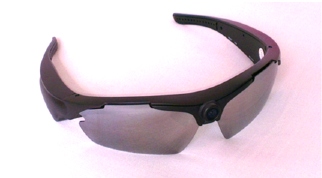
\includegraphics[width=0.95\textwidth]{images/Sonification1.png}
    \caption{vOICe device.}
    \label{fig:sonification1}
\end{figure}

There have also been attempts to create location devices as a replacement for guide dogs.
For example, Dr. Leslie Kay’s “Sonic Torch”, a device using traditional sonar technology, which uses a bat-like frequency sweep to return detailed textural information \cite*{Girvin2005}.
Another attempt at a location device is created by Dr. Peter Meijer and is called vOICe. 
This works by taking the input from a digital camera, either a mounted one or the camera from a cellphone, and using software to sweep the image with a vertical scan line. 
It then sonifies features in the scan by representing vertical position as pitch, horizontal position as time, and brightness by increasing or decreasing volume \cite*{Girvin2005}. 
An interesting result that came from using this device was that a user reported experiences of seeing depth in different places throughout her house. On Dr. Meijer website \url{www.seeingwithsound.com}, a demo of vOICe made in Java can be found. 
On here the application is mentioned as “Augmented Reality for the Totally Blind”. 
Figure~\ref{fig:sonification1} shows an example of how a vOICe device can look. 
The camera in the center is what captures the mage then processed as previously mentioned.
As a last example regarding blind users, Joshua Miele of the Smith Kettlewell Eye Research Institute in San Francisco has written braille support for MATLAB and the sonification toolbox for blind engineers and scientists~\cite*{Girvin2005}. 

% subsubsection examples_of_sonification (end)


\subsubsection{Sonification Techniques} % (fold)
\label{ssub:sonification_techniques}

One way of defining sonifications is describing them according to their sonification techniques.

\begin{enumerate}
    \item Event-based
    \item Model-based
    \item Continuous
\end{enumerate}

The appeal of de Campo’s(XX) approach is that it allows for blurry boundaries between the categories and offers guidance for choosing a sonification technique.


\subsubsection*{Interactivity} % (fold)
\label{ssub:interactivity}

One of the elements to consider when discussing sonification techniques is the interactivity available (or unavailable) to the user of an auditory display. 
Interactivity with auditory displays ranges from completely non-interactive to completely user initiated. 
Non-interactive sonification is often referred to as “concert mode”. 
Instances where the user is able to change and/or choose parameters of the display, has been referred to as “query based” or “conservation mode”. 
User input may also be the driving factor of the presentation of the sound. 

\begin{quote}
``For most sonifications to be useful there must at least be some sort of interactivity, even if it is just play/pause or replay of a certain sound.'' \cite*{Hermann2011}
\end{quote}

% subsubsection interactivity (end)


\subsubsection*{Parameter mapping (event-based sonification)} % (fold)
\label{ssub:parameter_mapping_event_based_sonification_}

``Parameter mapping represents changes in some data dimension with changes in an acoustic dimension to produce a sonification'' \cite*{Hermann2011}.
Sound has many changeable dimension such as frequency, amplitude, phase etc. 
The dimensionality of these data must however be constrained such that a perceivable display is feasible. 
The data changes may be discrete or qualitative. 
For instance, and alarm may be triggered by a discrete on or off threshold, or parameter mapping can be a series of discrete data which makes it seem more continuous. 
These event-based techniques have a passive mode of interaction. 
Some event-based sonifications are brief and offer limited opportunity for user input. 

% subsubsection parameter_mapping_event_based_sonification_ (end)


\subsubsection*{Model-based sonification} % (fold)
\label{ssub:model_based_sonification}

The model-based approach is different from the event-based approaches in that instead of mapping data parameters to sound parameters, the developer builds a virtual model whose sonic responses to user input is derived from data. 
A model is a virtual instrument with which the user can interact with. 
The user input drives the sonification. 
The user learns to understand the structure based on the sonic feedback of the user’s input. 
These types of sonification usually involves large numbers of data points and a high data dimensionality.

% subsubsection model_based_sonification (end)


\subsubsection*{Audification (continues sonification)} % (fold)
\label{ssub:audification_continues_sonification_}

Audification is a direct form of sonification where waveforms of periodic data are directly translated into sound. 
For instance, a Geiger counter gives the user constant sonic feedback of the radiation level by translating data of radiation level into sound.

% subsubsection audification_continues_sonification_ (end)

% subsubsection sonification_techniques (end)


\subsection{subsection name} % (fold)
\label{sub:subsection_name}

% subsection subsection_name (end)

% section preanalysis (end)
